\documentclass[xcolor=table, aspectratio=169,ignorenonframetext]{beamer}

%\usepackage{arev}
\usepackage{amsmath,amssymb,amscd}
\usepackage{dsfont}
\usepackage{mathrsfs}
\usepackage{yfonts}
\usepackage{bm}
\usepackage{graphicx}
\usepackage{tabularx}
\usepackage{animate}
\usepackage{listings}
%\usepackage{ifthen}
\usepackage{pifont}

\usepackage{xeCJK}
\usepackage{fontspec}
\newfontfamily\cjkfont{WenQuanYi Zen Hei}
\setCJKmainfont{WenQuanYi Zen Hei}
%\newfontfamily\cjkfont{PingFang SC}
%\setCJKmainfont{PingFang SC}
\newcolumntype{x}{>{\centering\arraybackslash}X}
\renewcommand{\arraystretch}{1.5}
\DeclareMathOperator{\img}{img}
\DeclareMathOperator{\hhom}{Hom}
\newcommand{\uone}{\text U(1)}
\DeclareMathOperator{\id}{id}
\usepackage{tikz}
	\usetikzlibrary{calc}
	\usetikzlibrary{arrows,shapes, positioning, matrix}
	\usetikzlibrary{decorations.markings}
	\tikzstyle arrowstyle=[scale=1]
  \tikzstyle string=[thick,postaction={decorate,decoration={markings,
      mark=at position .55 with {\arrow[arrowstyle]{stealth}}}}]

\usepackage{tikz-cd}
\usepackage{pgffor}
\newcommand{\cohosub}[1]{\scalebox{0.72}{\textswab{#1}}}
\newcommand{\cohosubsub}[1]{\scalebox{0.6}{\textswab{#1}}}
\newcommand{\coho}[1]{\textswab{#1}}


\mode<presentation>
{
  %\usetheme{Warsaw}
  % or ...
  %\useoutertheme{rectangle}
  \setbeamertemplate{frametitle}[default][center]
  \defbeamertemplate{itemize item}{flat}{\begin{pgfpicture}{-1ex}{0ex}{1ex}{2ex}
      \pgfpathcircle{\pgfpoint{0pt}{.6ex}}{0.6ex}
      \pgfusepath{fill}
    \end{pgfpicture}%
  }
  \defbeamertemplate{itemize subitem}{flat}{\footnotesize\raise0.5pt\hbox{\textbullet}}
  \defbeamertemplate{itemize subsubitem}{flat}{\footnotesize\raise0.5pt\hbox{\textbullet}}

  %\useinnertheme{circles}
  \setbeamertemplate{items}[flat]
  \setbeamertemplate{sections/subsections in toc}[circle]
  \setbeamertemplate{blocks}[rounded]
  \setbeamertemplate{title page}[default][colsep=-4bp,rounded=true]
  \setbeamertemplate{part page}[default][colsep=-4bp,rounded=true]
  \setbeamercovered{transparent}
  %\usecolortheme{spruce}
  %\definecolor{THU}{RGB}{116,61,130}
  \definecolor{mbg}{RGB}{0,0,160}
  \setbeamercolor*{palette primary}{fg=white,bg=mbg}
  \setbeamercolor*{titlelike}{parent=palette primary}
  \setbeamercolor*{structure}{fg=mbg}
  \setbeamercolor{frametitle}{fg=white,bg=mbg}
  % or whatever (possibly just delete it)
  \setbeamercolor{block title}{bg=mbg,fg=white}
  \setbeamercolor{block body}{bg=mbg!15}


  \addtobeamertemplate{navigation symbols}{}{ \hspace{1em}%
    \usebeamerfont{footline}%
    \insertframenumber / \inserttotalframenumber }
}


%\usepackage[english]{babel}
% or whatever

%\usepackage[latin1]{inputenc}
% or whatever

%\usepackage{times}
%\usepackage[T1]{fontenc}
% Or whatever. Note that the encoding and the font should match. If T1
% does not look nice, try deleting the line with the fontenc.

\title % (optional, use only with long paper titles)
{Emergent U(1) symmetry and BKT transition in a triangular-lattice quantum Ising material TmMgGaO${}_4$}
\author[Y Qi] % (optional, use only with lots of authors)
{Yang~Qi}
% - Give the names in the same order as the appear in the paper.
% - Use the \inst{?} command only if the authors have different
%   affiliation.

\institute[Fudan] % (optional, but mostly needed)
{
Department of Physics, Fudan University.
}
% - Use the \inst command only if there are several affiliations.
% - Keep it simple, no one is interested in your street address.

%\date{2016 Annual Meeting of Fudan CFTPP} % (optional, should be abbreviation of conference name)
%{Fudan University, Oct 13 2015}
\date{Oct. 17th, 2020}
% - Either use conference name or its abbreviation.
% - Not really informative to the audience, more for people (including
%   yourself) who are reading the slides online

%\subject{Theoretical Physics}
% This is only inserted into the PDF information catalog. Can be left
% out.



% If you have a file called "university-logo-filename.xxx", where xxx
% is a graphic format that can be processed by latex or pdflatex,
% resp., then you can add a logo as follows:

\pgfdeclareimage[height=1cm]{university-logo}{../resources/fudan}
\logo{\pgfuseimage{university-logo}}



% Delete this, if you do not want the table of contents to pop up at
% the beginning of each subsection:
\AtBeginSection[]
{
  \begin{frame}<beamer>{Outline}
			\tableofcontents[currentsection,currentsubsection]
  \end{frame}
}
%\AtBeginSubsection[]
%{
 % \begin{frame}<beamer>{Outline}
  %  \tableofcontents[currentsection,currentsubsection]
  %\end{frame}
%}


\begin{document}

\begin{frame}
  \titlepage
\end{frame}

\begin{frame}{Collaborators: Beihang University}
\begin{itemize}
	\item XTRG: Han Li (李涵), Bin-Bin Chen (陈斌斌), Wei Li (李伟).
	\item DFT: Xu-Tao Zeng, Xian-Lei Sheng (胜献雷).
\end{itemize}
	\begin{center}
		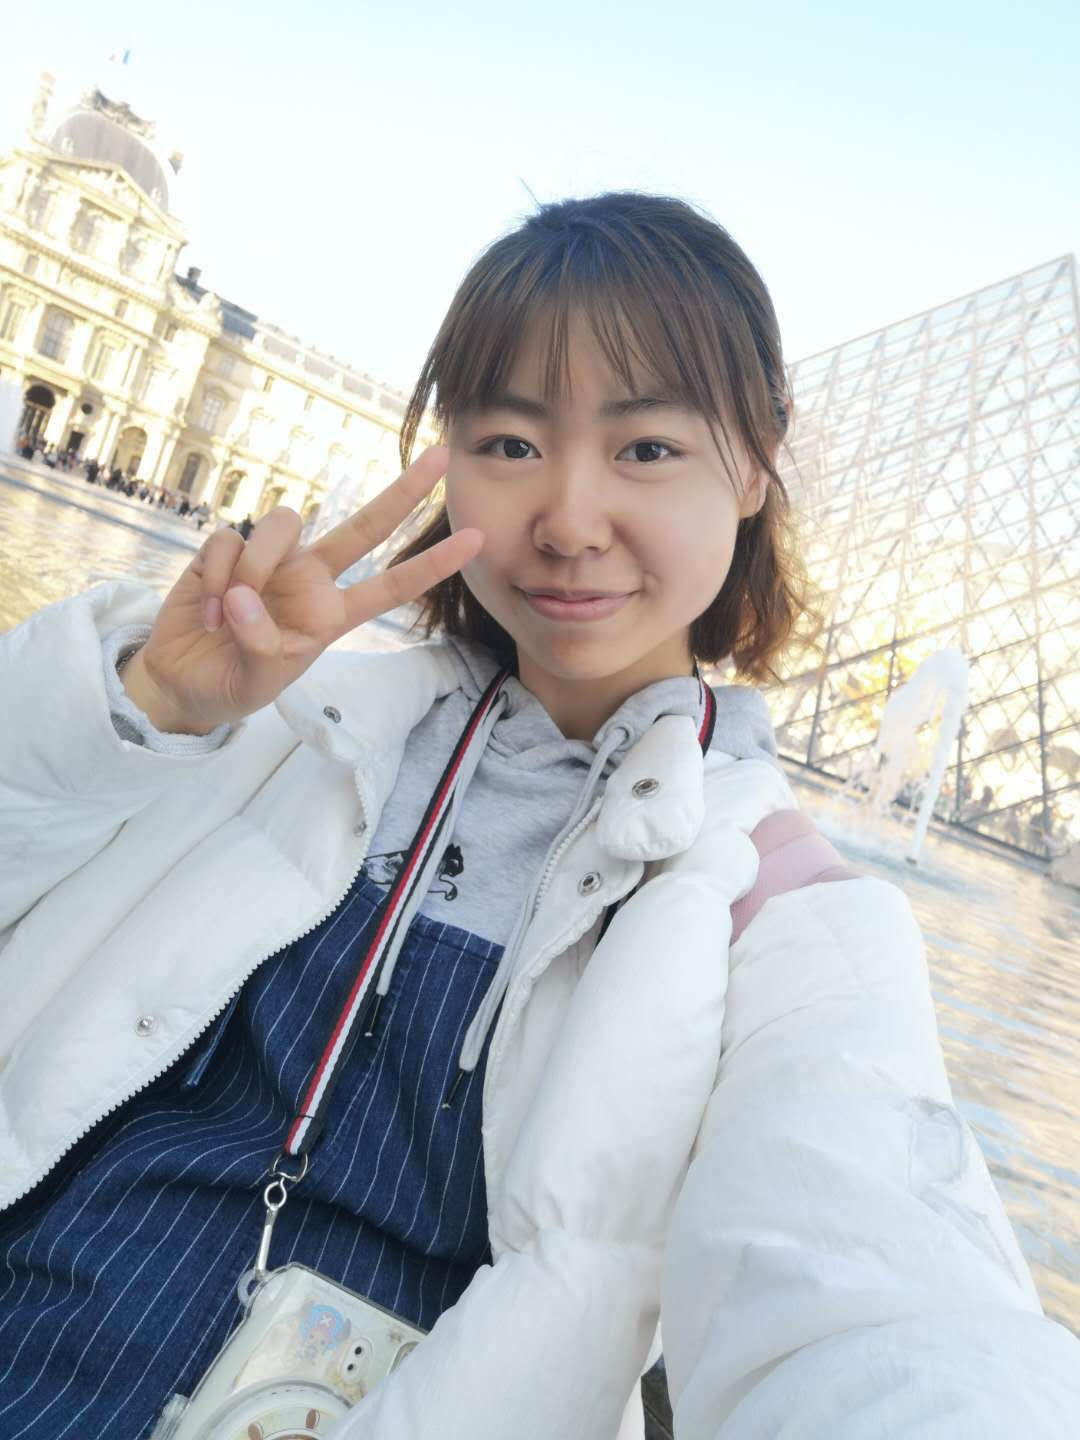
\includegraphics[height=3cm]{../people/hanli}
		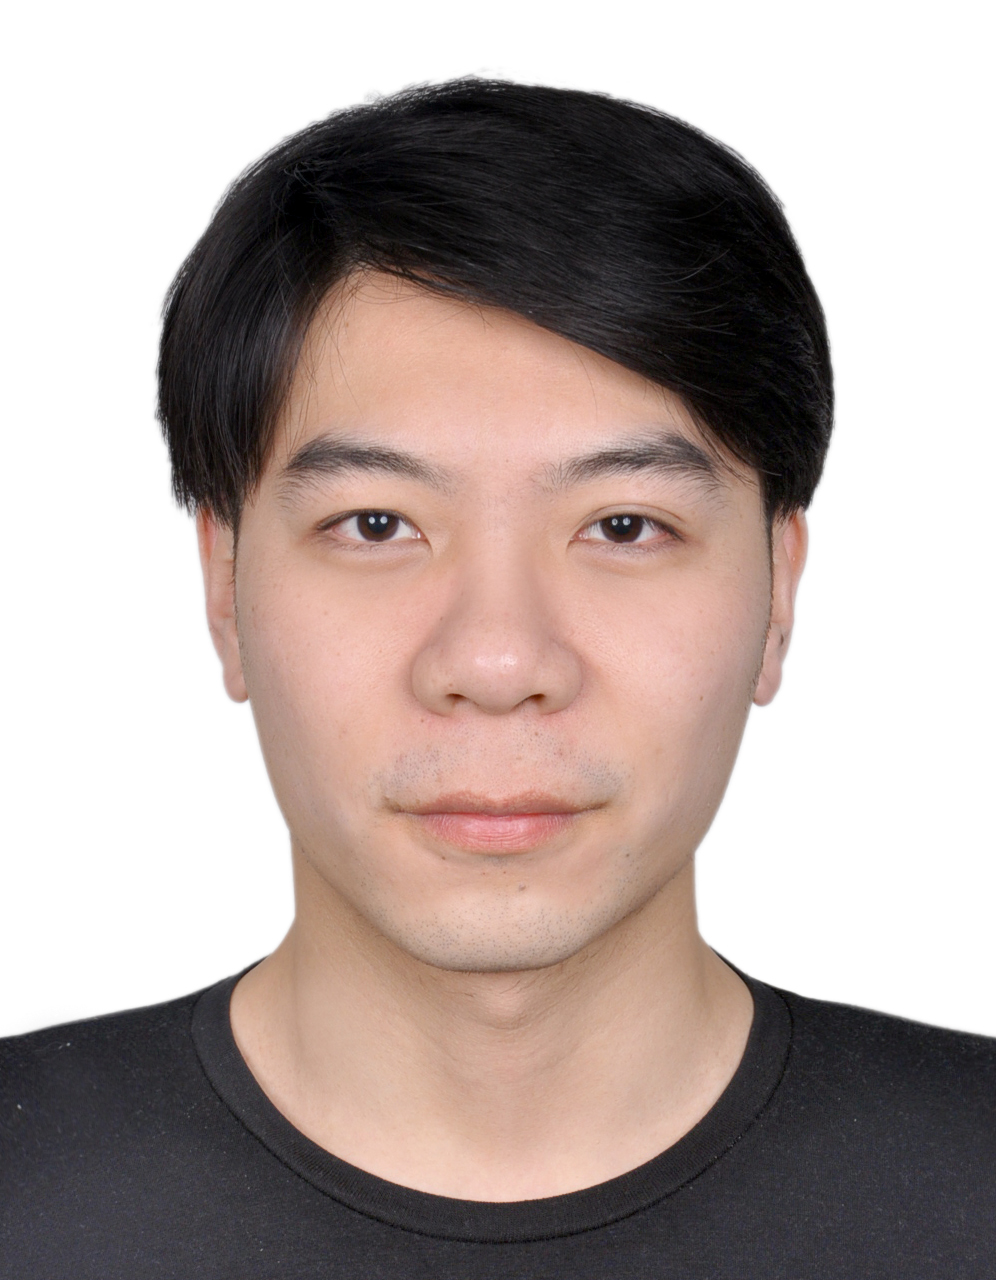
\includegraphics[height=3cm]{../people/binbinchen}
		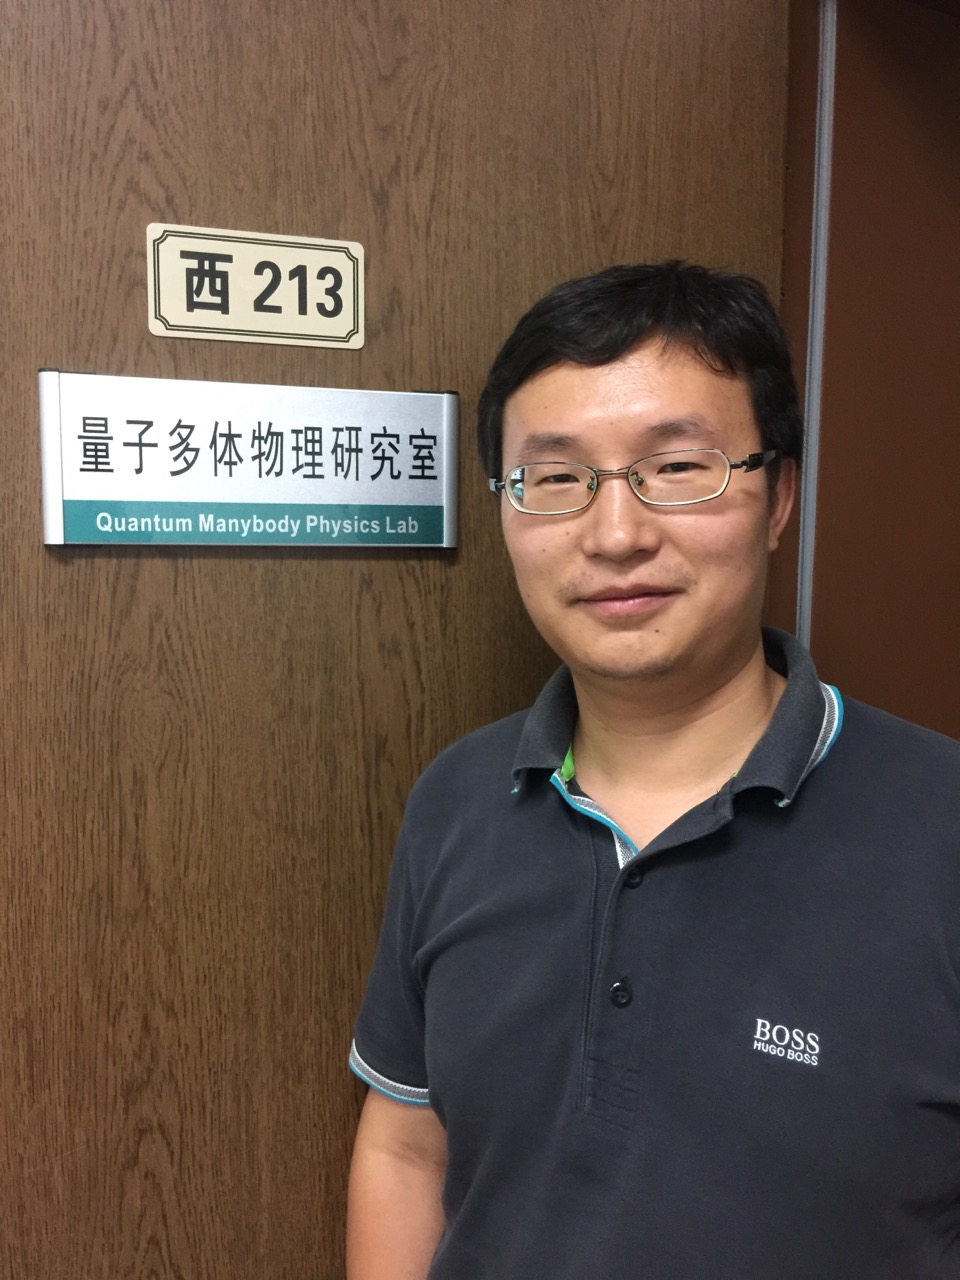
\includegraphics[height=3cm]{../people/weili}~~~~
		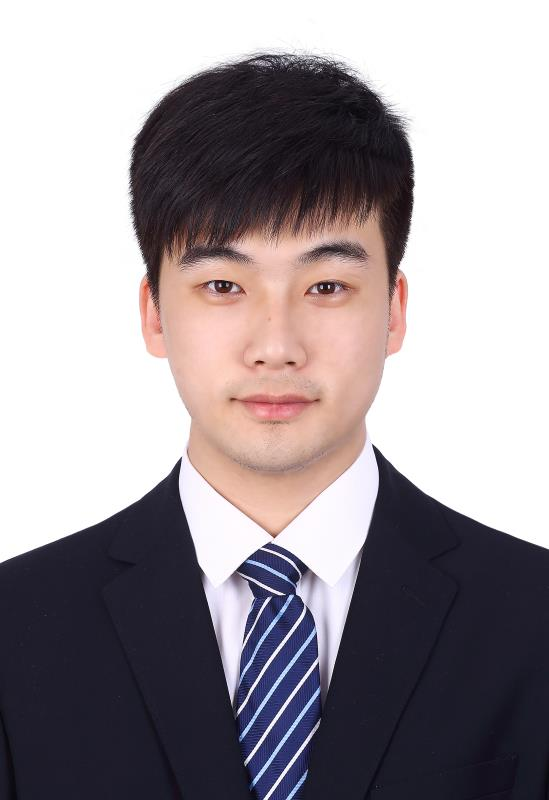
\includegraphics[height=3cm]{../people/xutaozeng}
		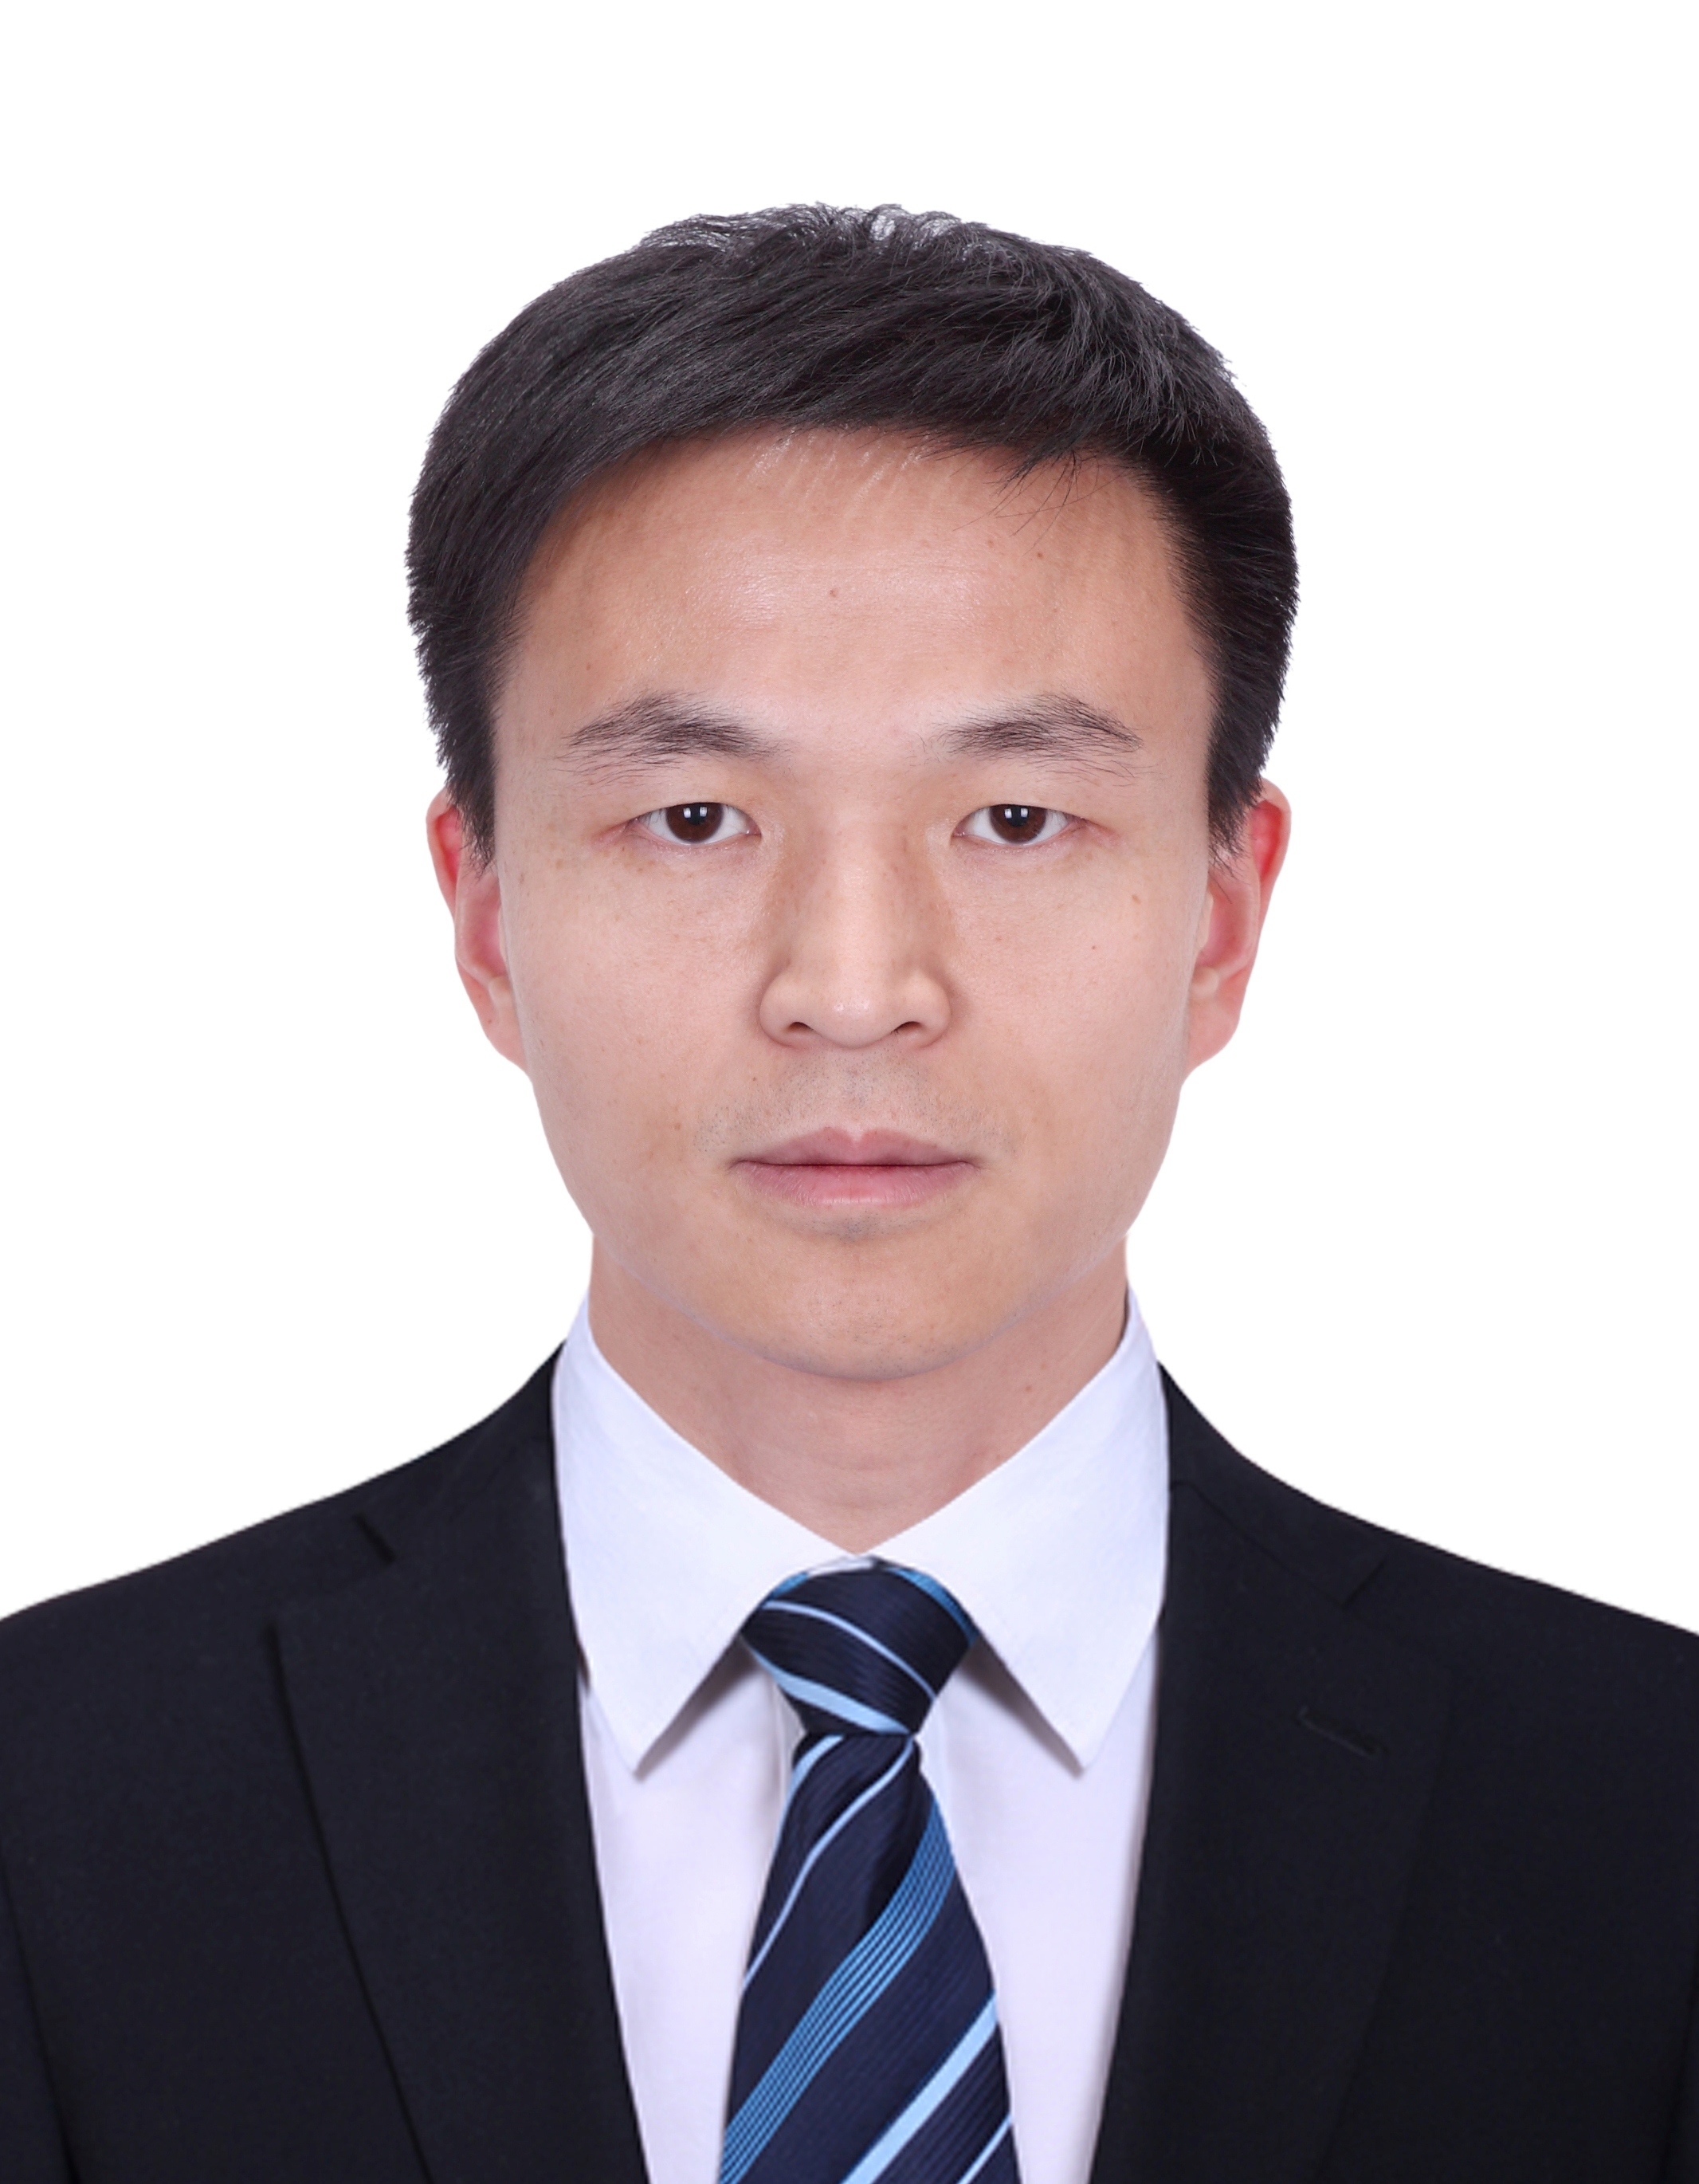
\includegraphics[height=3cm]{../people/xianleisheng}
	\end{center}
\end{frame}

\begin{frame}{Collaborators: Hong Kong University and Institute of Physics, CAS}
\begin{itemize}
	\item IOP, CAS: Yuan-Da Liao (廖元达).
	\item HKU: Zi Yang Meng (孟子杨).
	\item Quantum Monte Carlo simulations.
\end{itemize}
	\begin{center}
		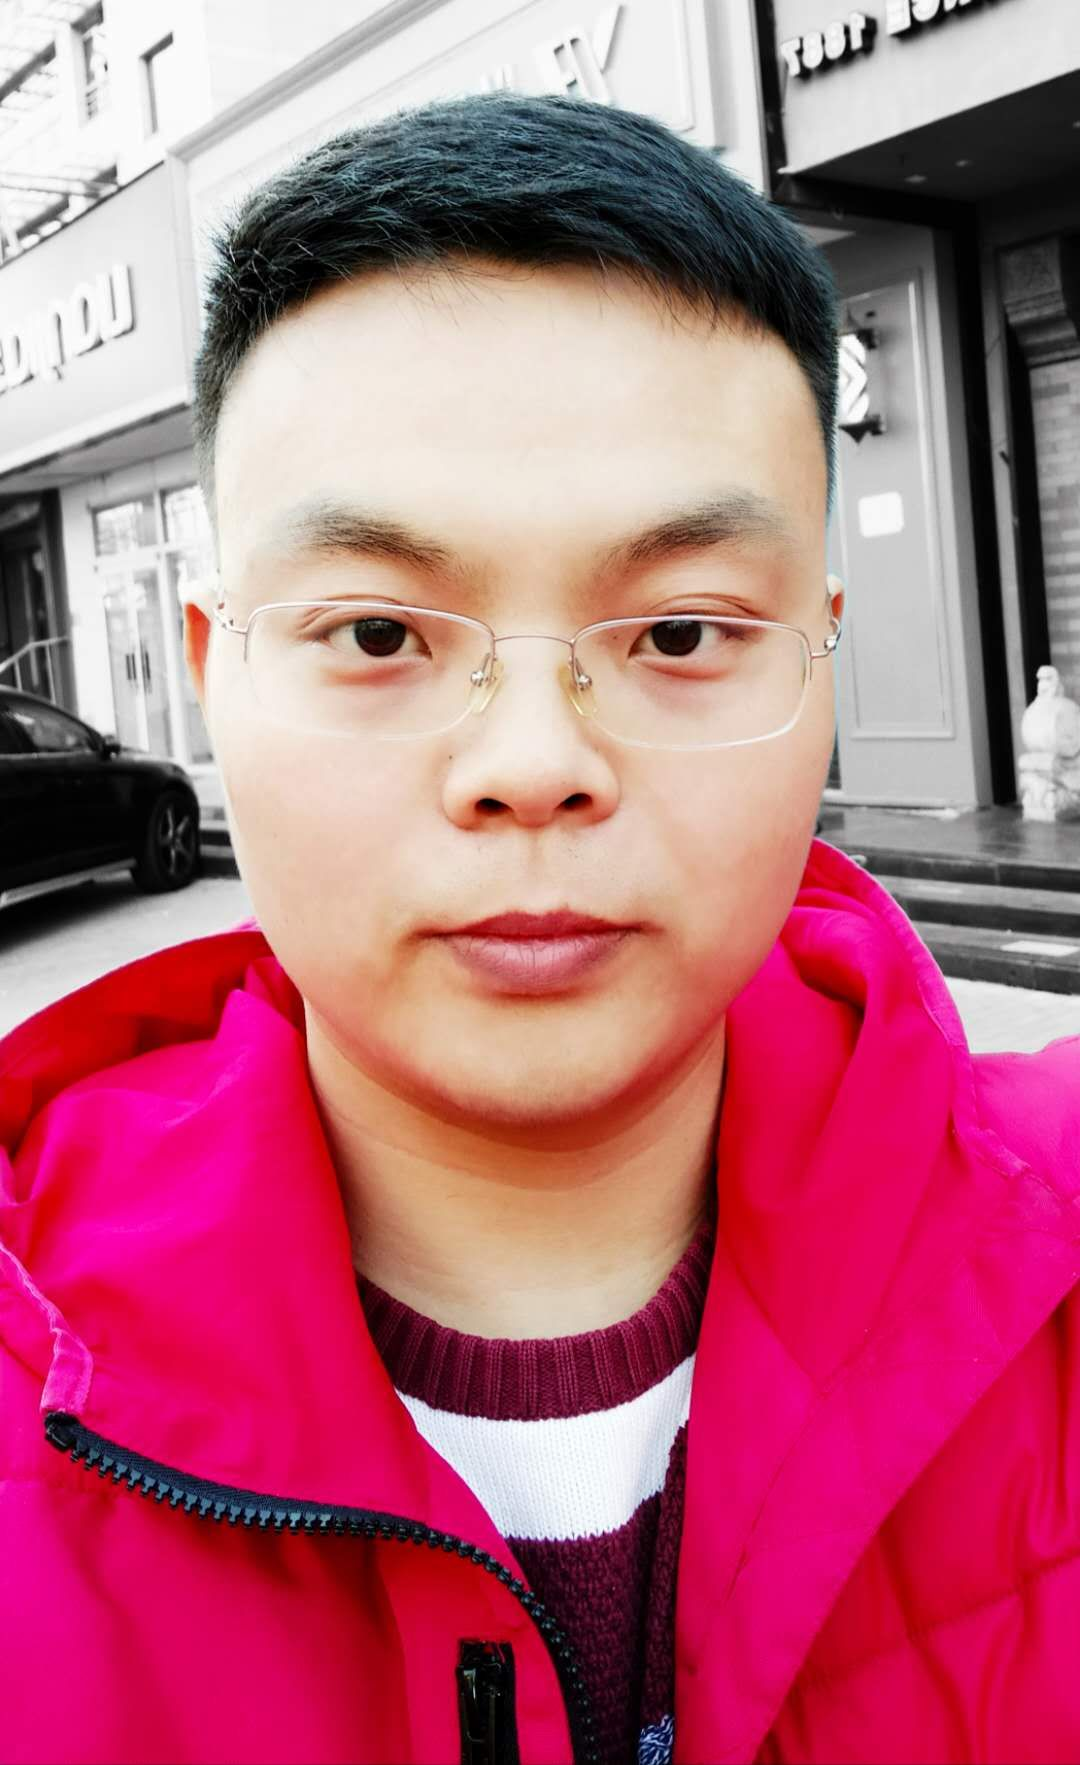
\includegraphics[height=3cm]{../people/yuandaliao}
		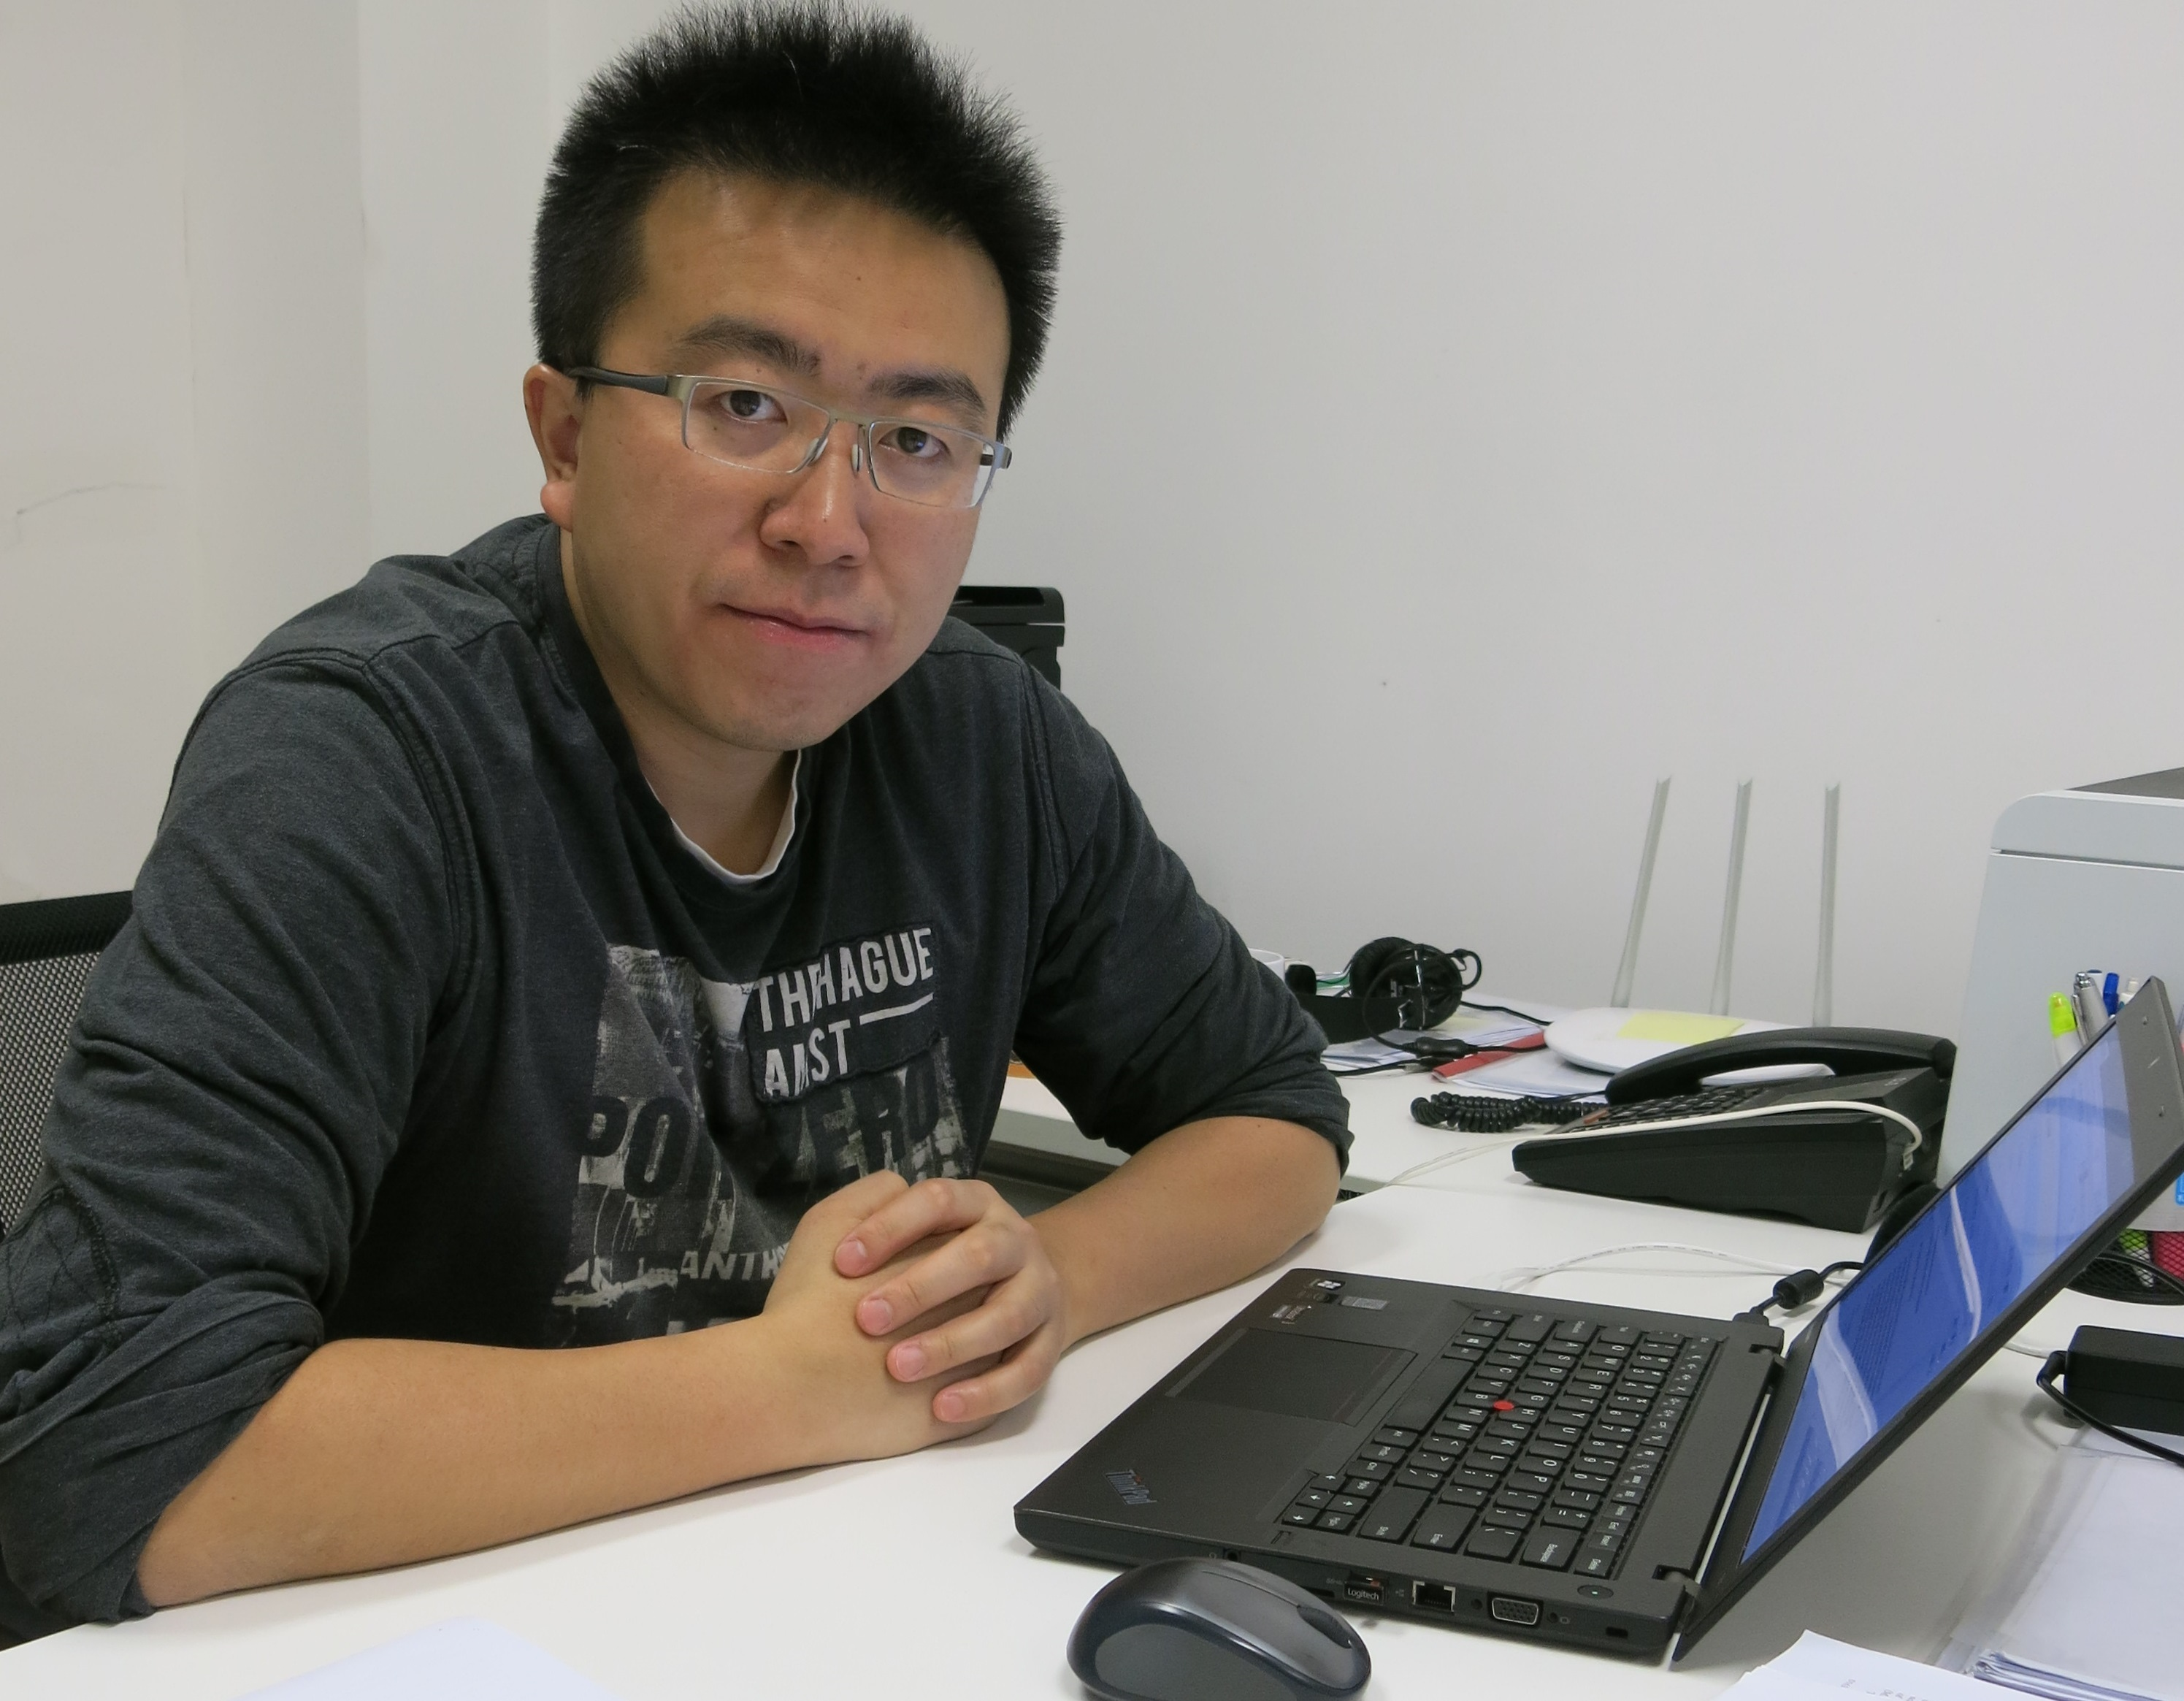
\includegraphics[height=3cm]{../people/ziyangmeng}
	\end{center}
\end{frame}

\begin{frame}{Collaborators: Renmin University}
\begin{itemize}
	\item Ze Hu (胡泽), Chunsheng Ma (马春生), Yi Cui (崔祎), Weiqiang Yu (于伟强).
	\item NMR measurement and susceptibility measurements.
\end{itemize}
	\begin{center}
		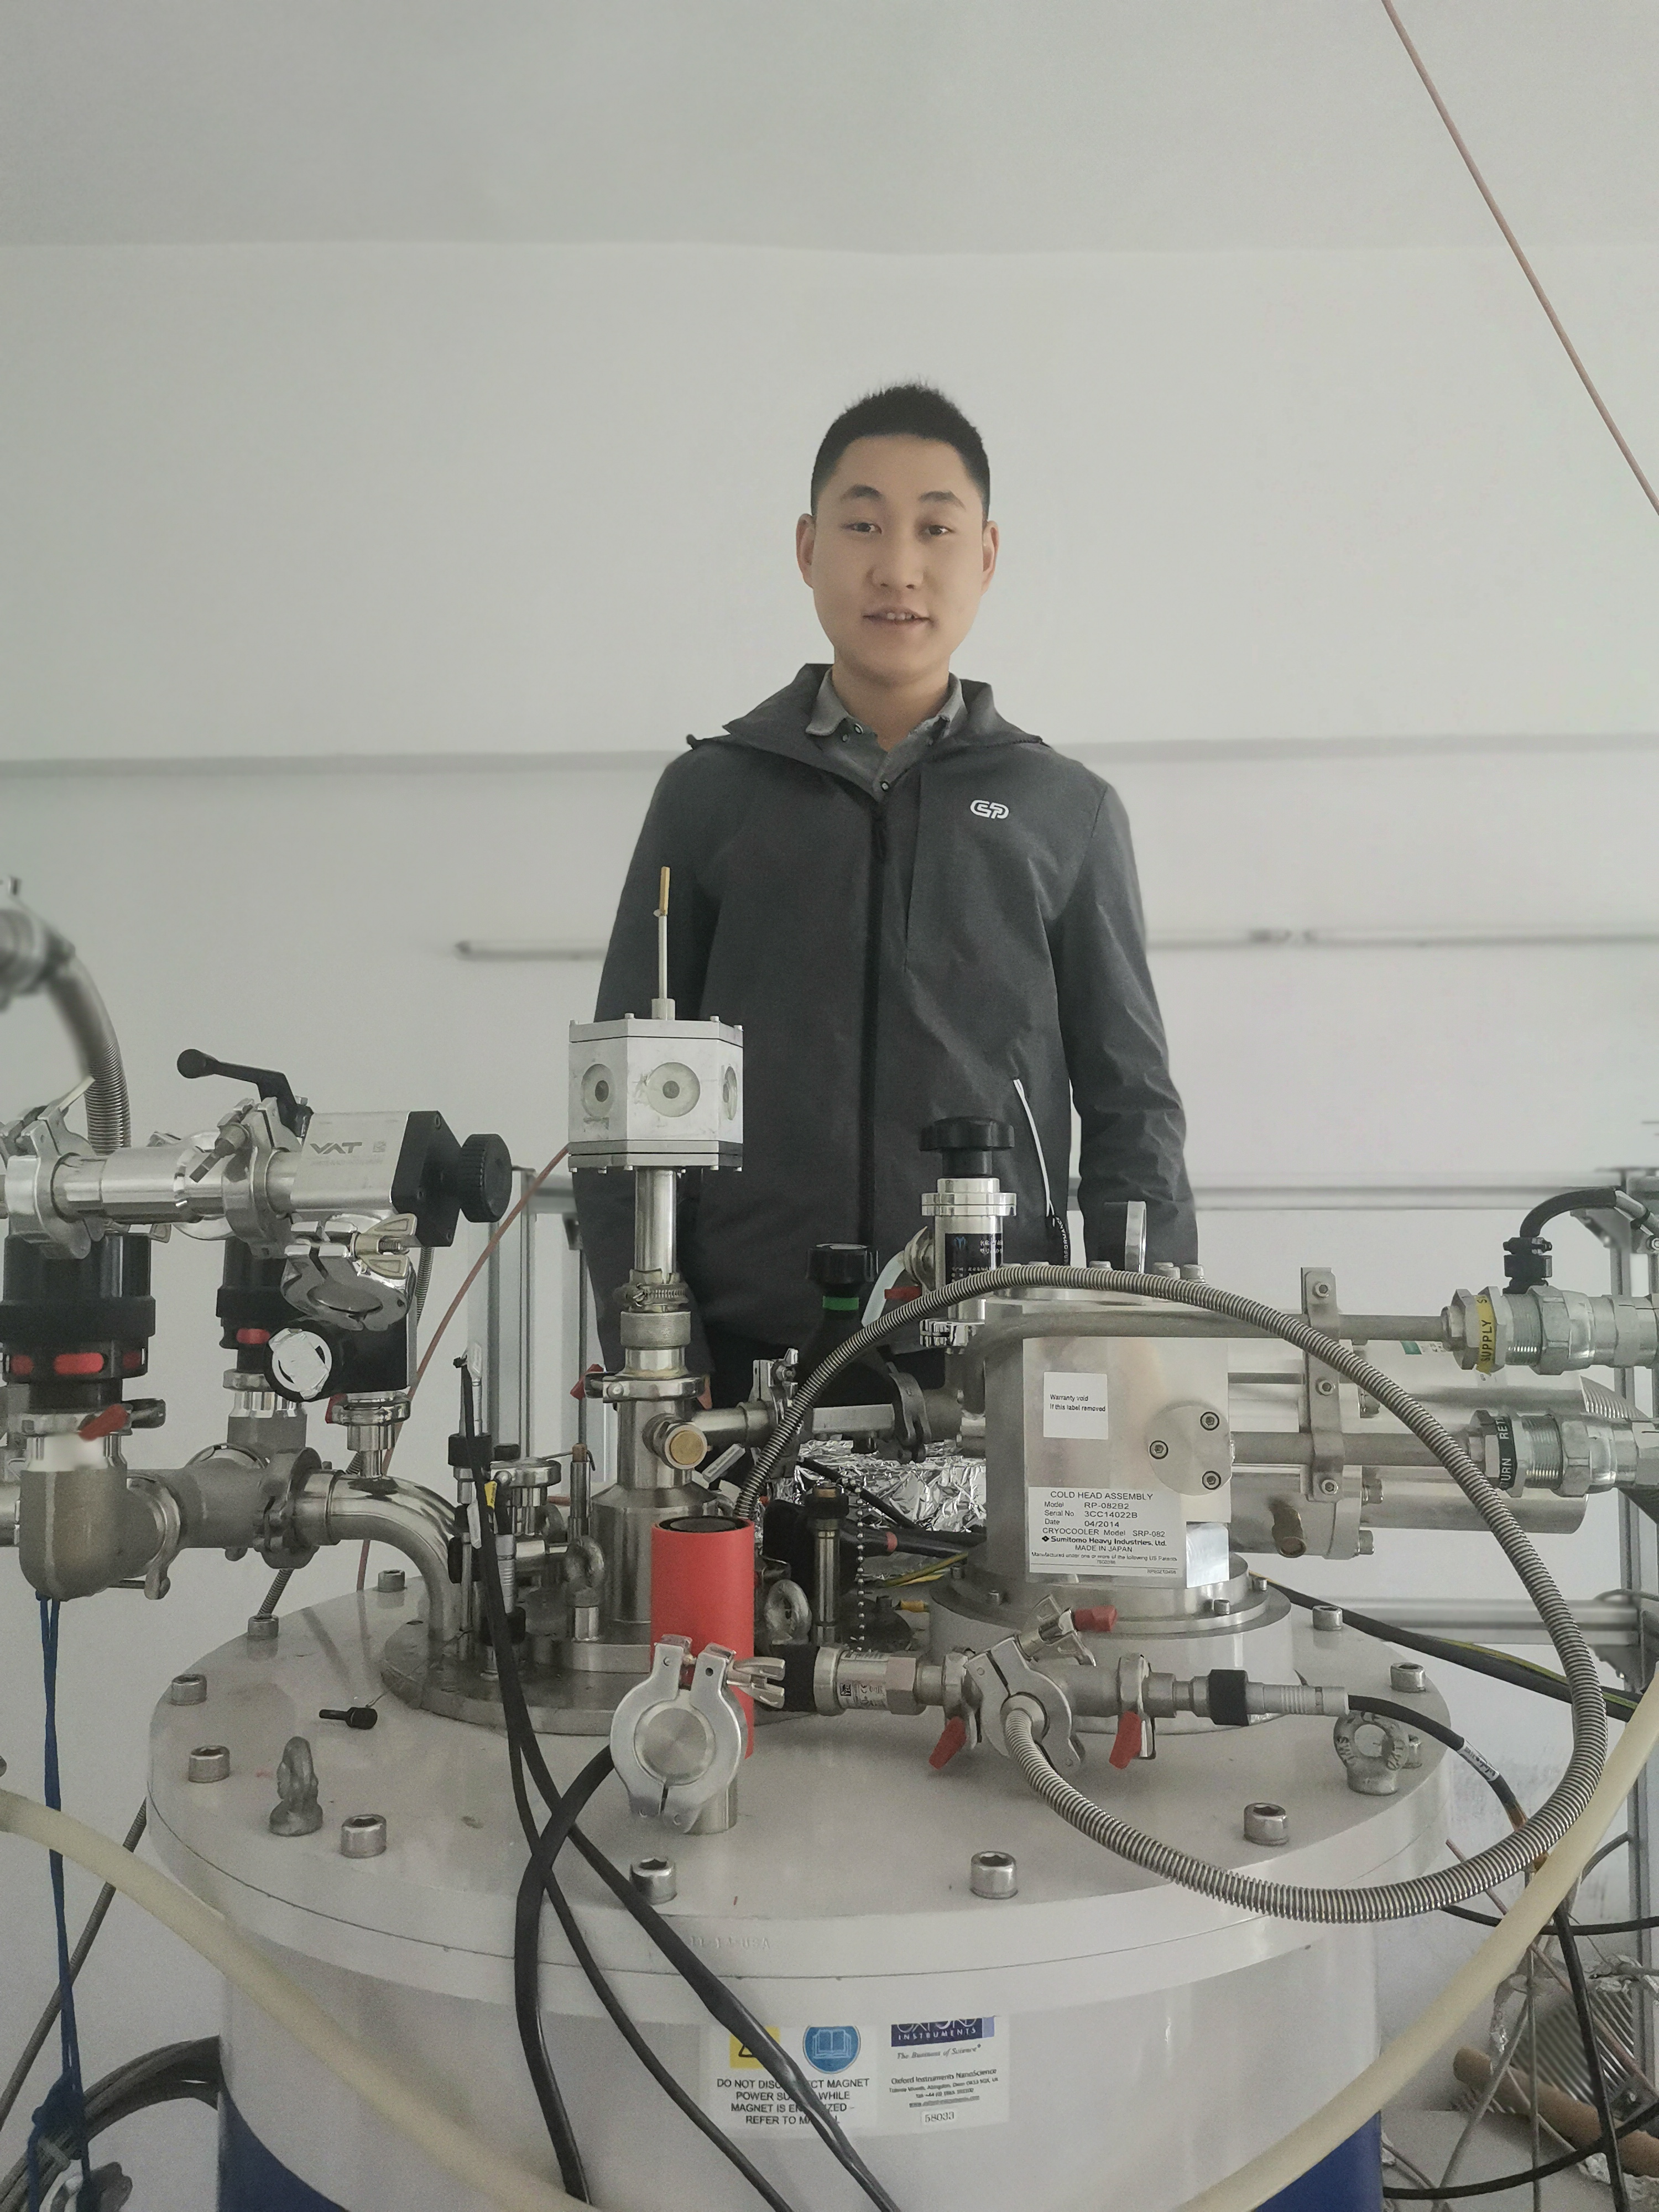
\includegraphics[height=5cm]{../people/zehu_large}
		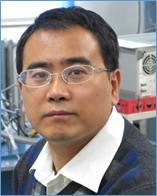
\includegraphics[height=5cm]{../people/weiqiangyu}
	\end{center}
\end{frame}

\begin{frame}{Collaborators: Nanjing University}
\begin{itemize}
	\item Zhen Ma (马祯), Yanyan Shangguan (上官艳艳), Zhentao Huang (黄振涛), Jinsheng Wen (温锦生).
	\item Single-crystal growth and susceptibility measurements.
\end{itemize}
	\begin{center}
		%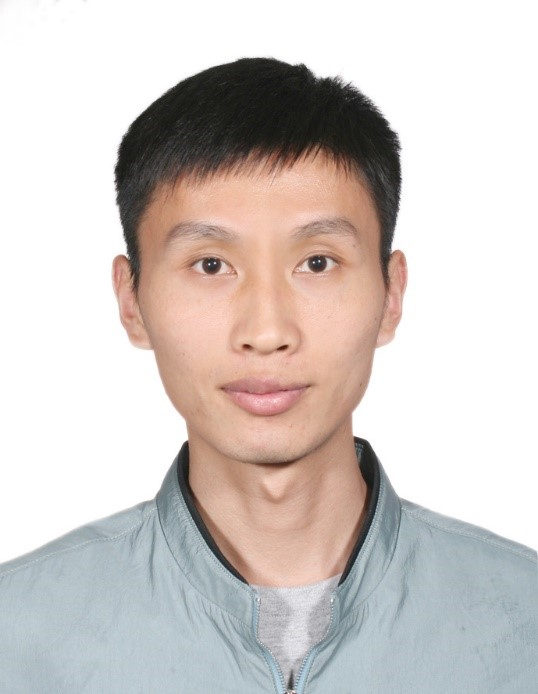
\includegraphics[height=5cm]{../people/zhenma}
		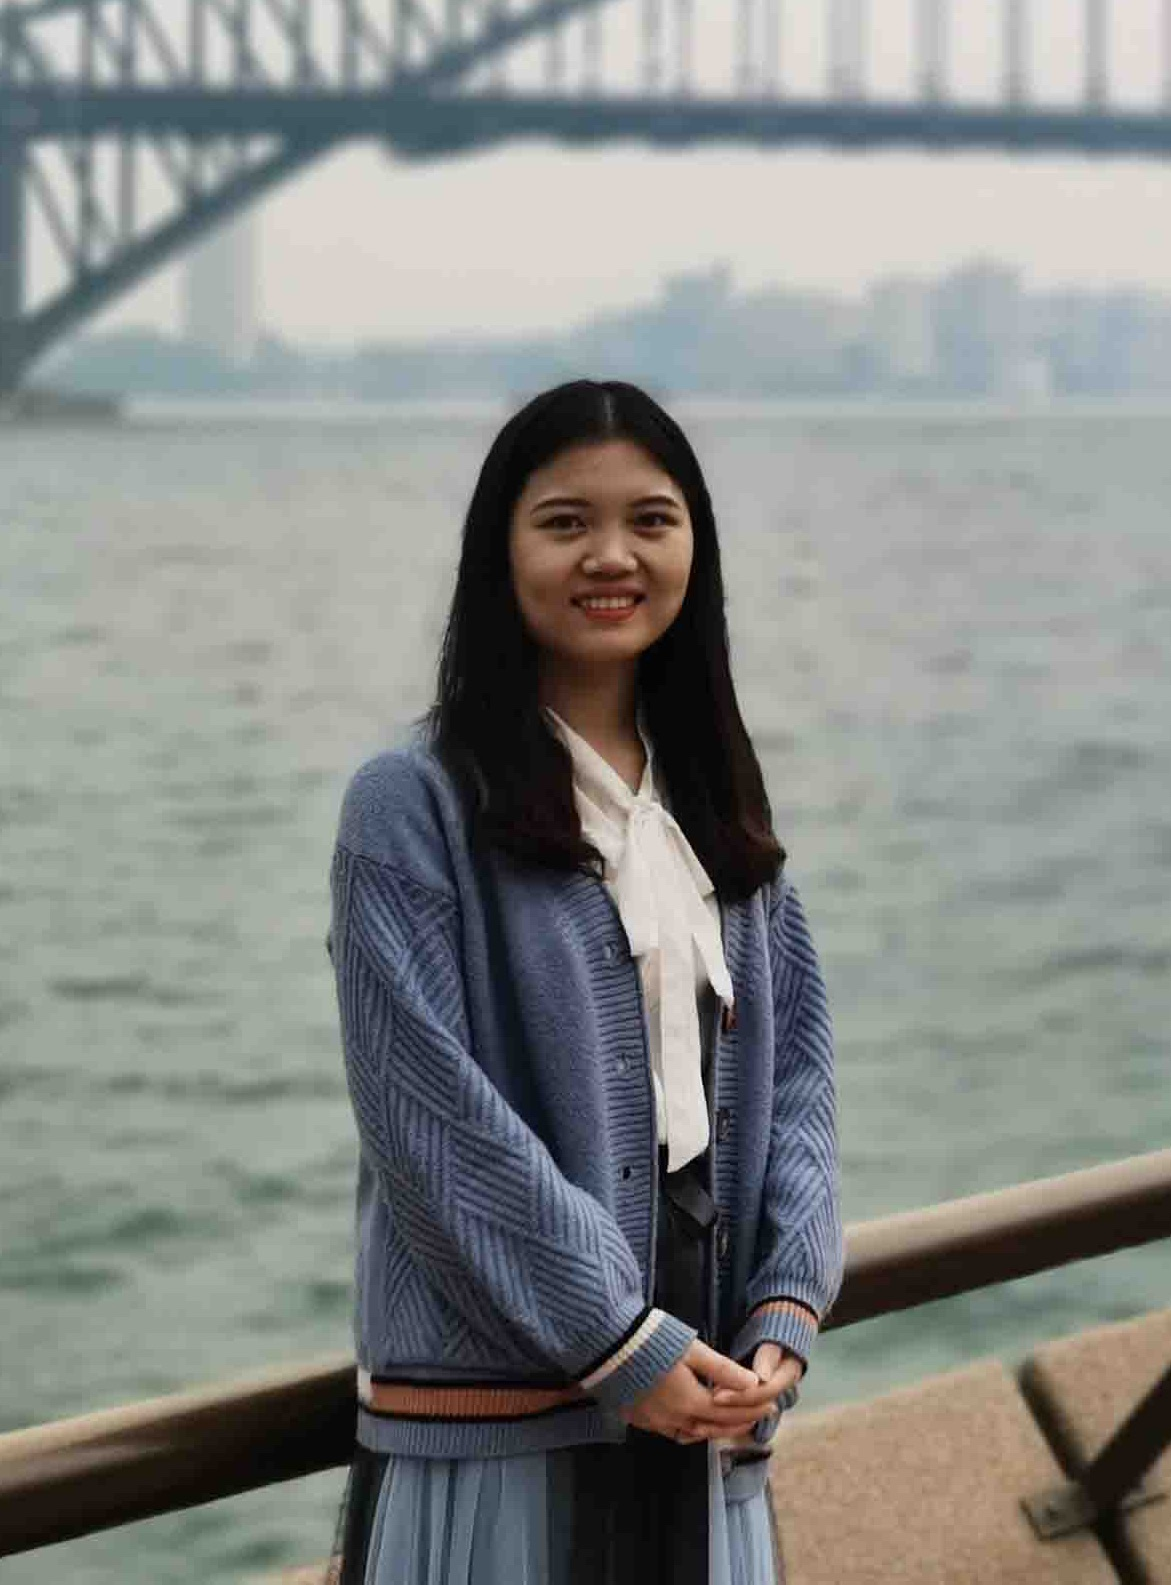
\includegraphics[height=3cm]{../people/yanyanshangguan}
		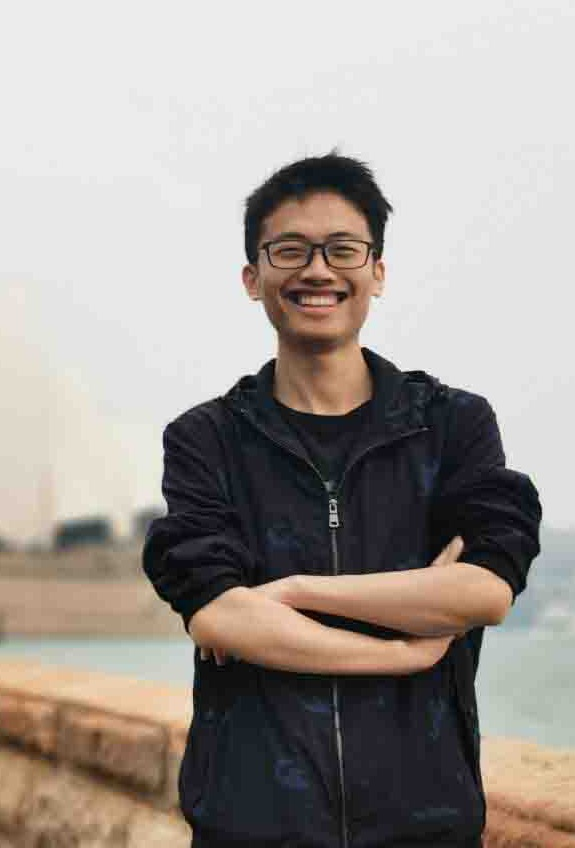
\includegraphics[height=3cm]{../people/zhentaohuang}
		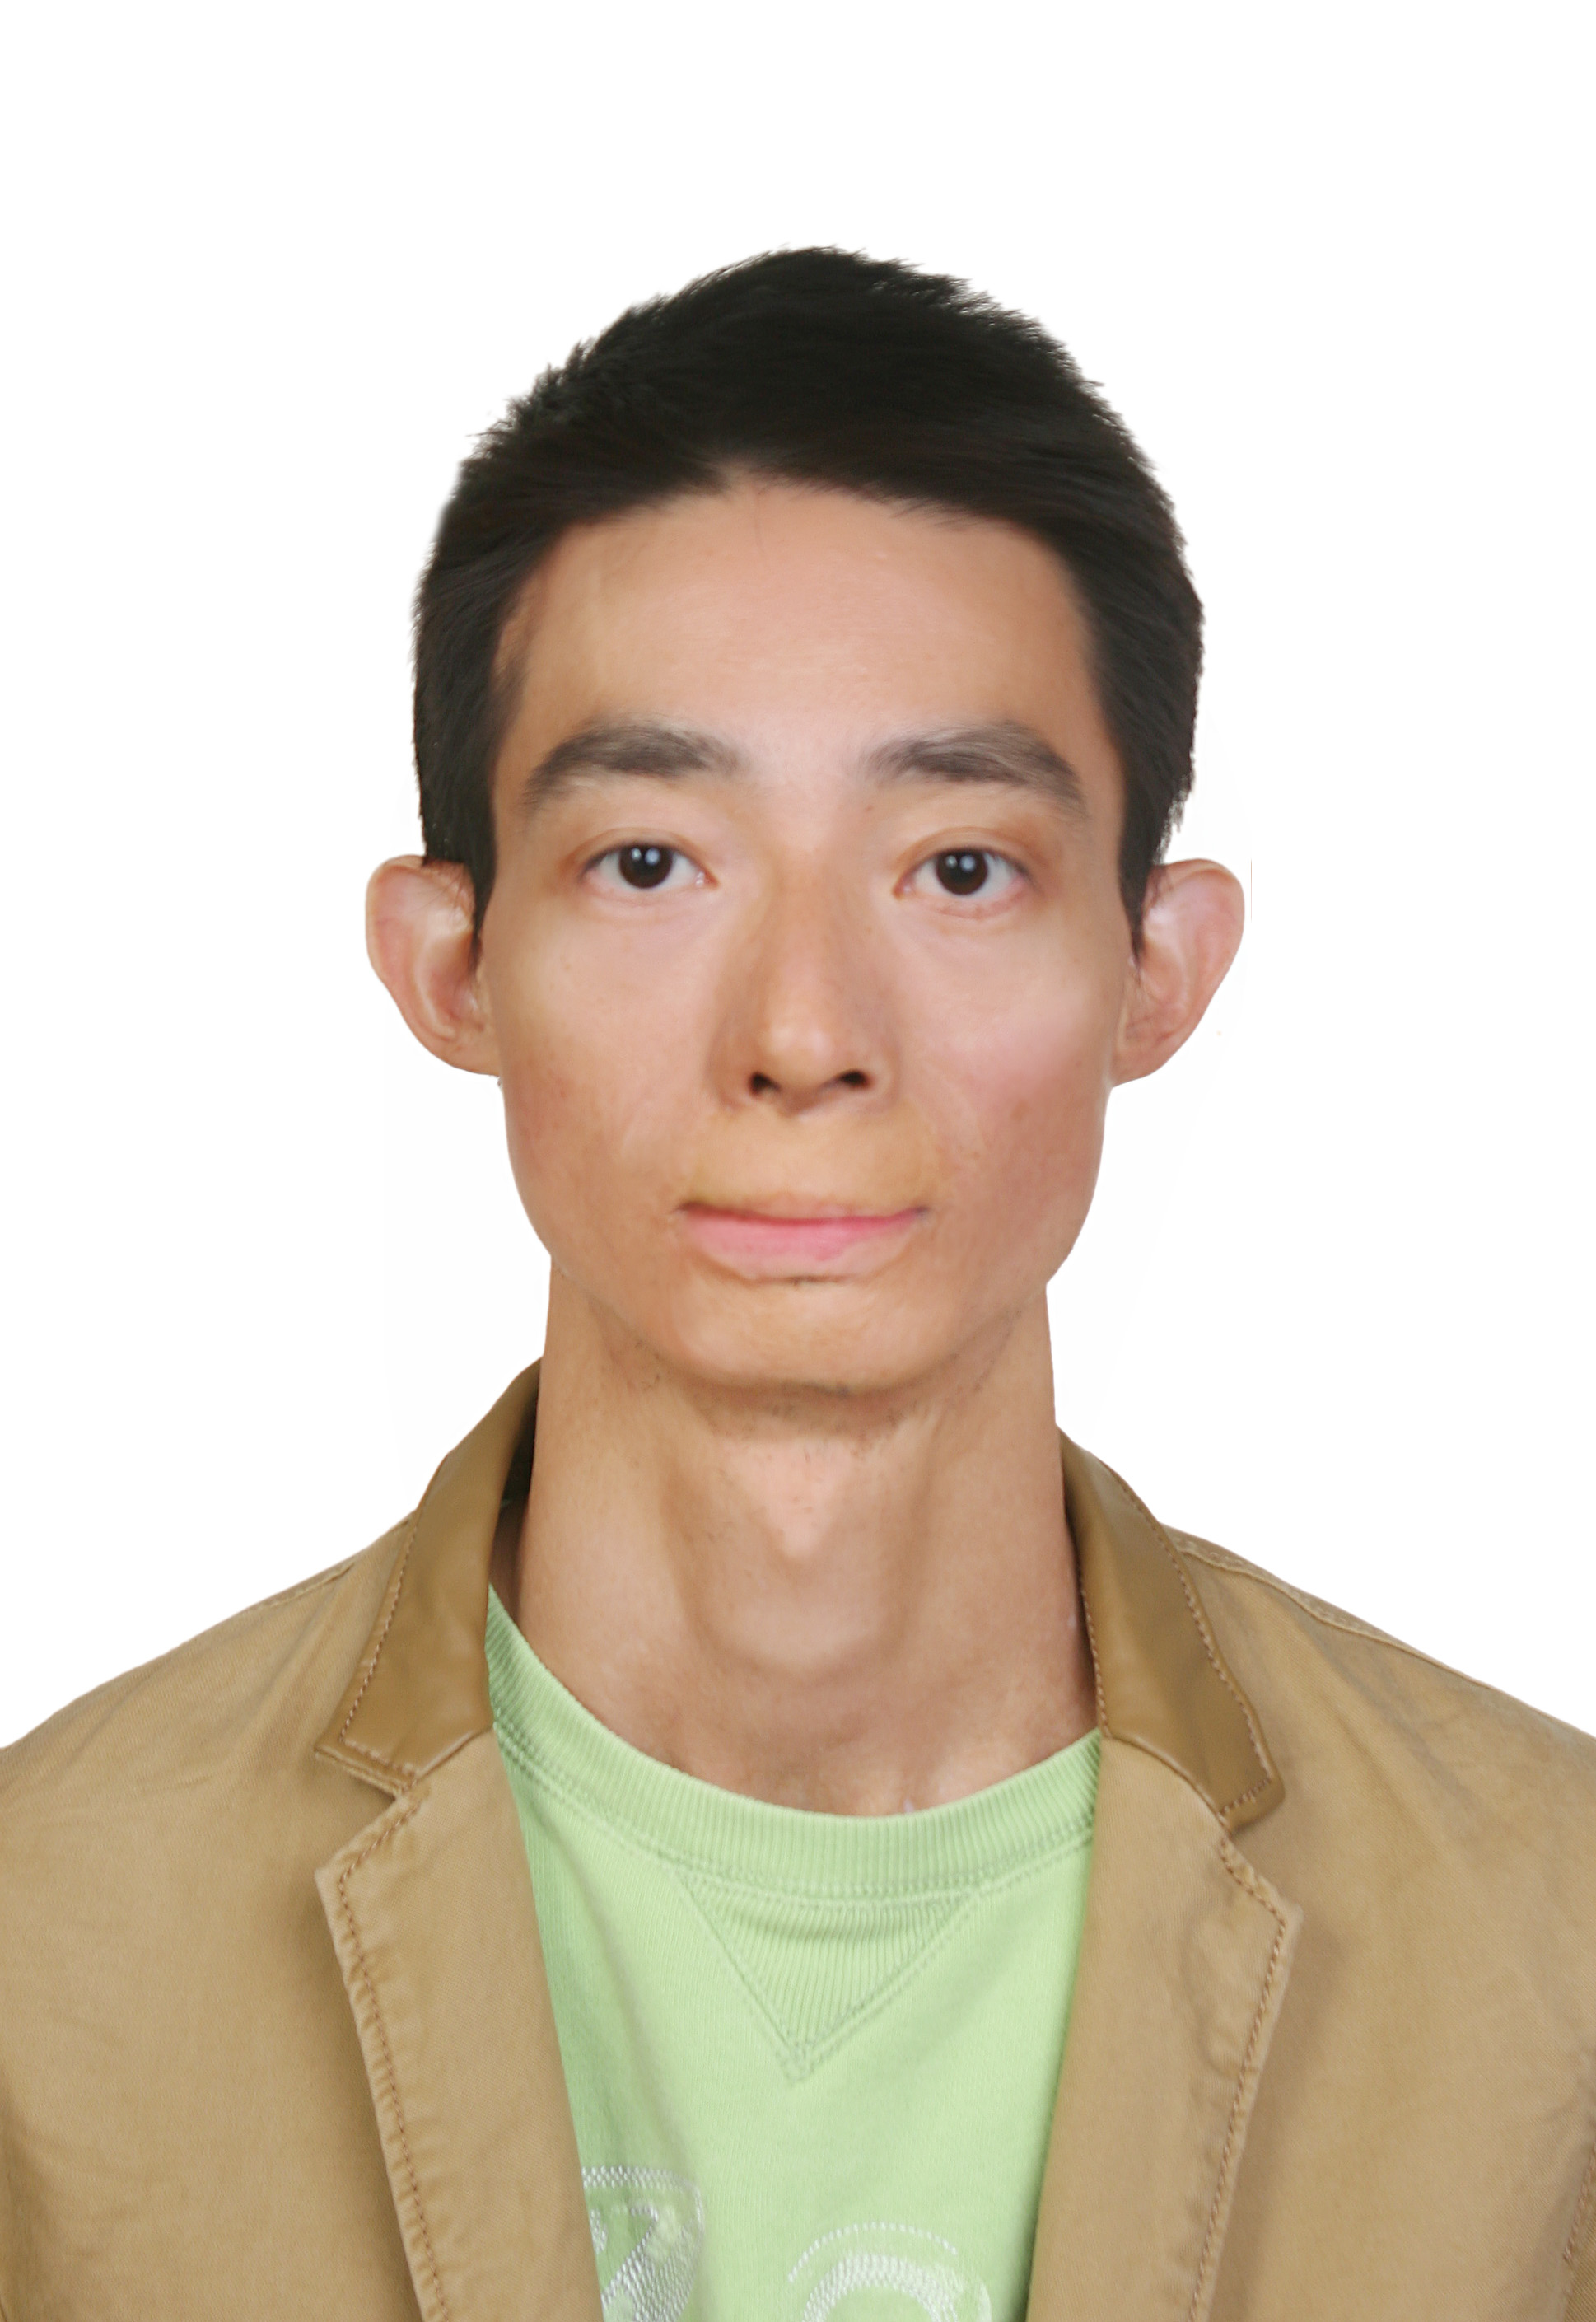
\includegraphics[height=3cm]{../people/jinshengwen}
	\end{center}
\end{frame}

\begin{frame}{References}
\begin{itemize}
	\item Evidence of the Berezinskii-Kosterlitz-Thouless phase in a frustrated magnet\\
Ze Hu\#, Zhen Ma\#, Yuan-Da Liao\#, Han Li\#, Chunsheng Ma, Yi Cui, Yanyan Shangguan, Zhentao Huang, Yang Qi*, Wei Li*, Zi Yang Meng*, Jinsheng Wen*, and Weiqiang Yu*\\
Nature Communications \textbf{11} 5631 (2020).
	\item Kosterlitz-Thouless melting of magnetic order in the triangular quantum Ising material TmMgGaO${}_4$\\
Han Li\#, Yuan Da Liao\#, Bin-Bin Chen, Xu-Tao Zeng, Xian-Lei Sheng, Yang Qi*, Zi Yang Meng*, and Wei Li*\\
Nature Communications \textbf{11}, 1111 (2020)
\end{itemize}
\end{frame}

\begin{frame}{Outline}
	%\begin{columns}
	%\column{.7\textwidth}
		\tableofcontents
  %\end{columns}
  % You might wish to add the option [pausesections]
\end{frame}

\section{Introduction: BKT transition}

\begin{frame}
	\frametitle{Landau's paradigm: universality class and symmetry breaking}
	\begin{itemize}
		\item Phases are classified by symmetry breaking.
		\item Continuous phase transitions = spontaneous symmetry breaking.
		\item Universality class is determined by symmetry group and dimensionality.
	\end{itemize}
\end{frame}

\begin{frame}
	\frametitle{BKT transition: classical exception to Landau's paradigm}
	\begin{itemize}
		\item Mermin-Wagner Thm:\\a continuous symmetry cannot be broken at finite-$T$ in $D\leq2$.
		\item Exception: U(1) symmetry in 2D.
	\end{itemize}
\end{frame}

\begin{frame}
	\frametitle{Realization of BKT transition}
	\begin{itemize}
		\item 2D superfluid (thin film).
		\item 2D superconductor (thin film).
		\item 2D ultracold bose gas.
		\item[?] Quantum magnets: 2D XY model?
		\[H=-J\sum_{\langle ij\rangle}\left(S_i^xS_j^x + S_i^yS_j^y\right).\]
	\end{itemize}
\end{frame}

\section{Material: From TmMgGaO${}_4$ to transverse-field Ising model}

\begin{frame}
	\frametitle{Effective DOF: Dipole-multipole doublet of Tm${}^{3+}$ ion}
	\begin{columns}
		\column{.6\textwidth}
		\begin{center}
			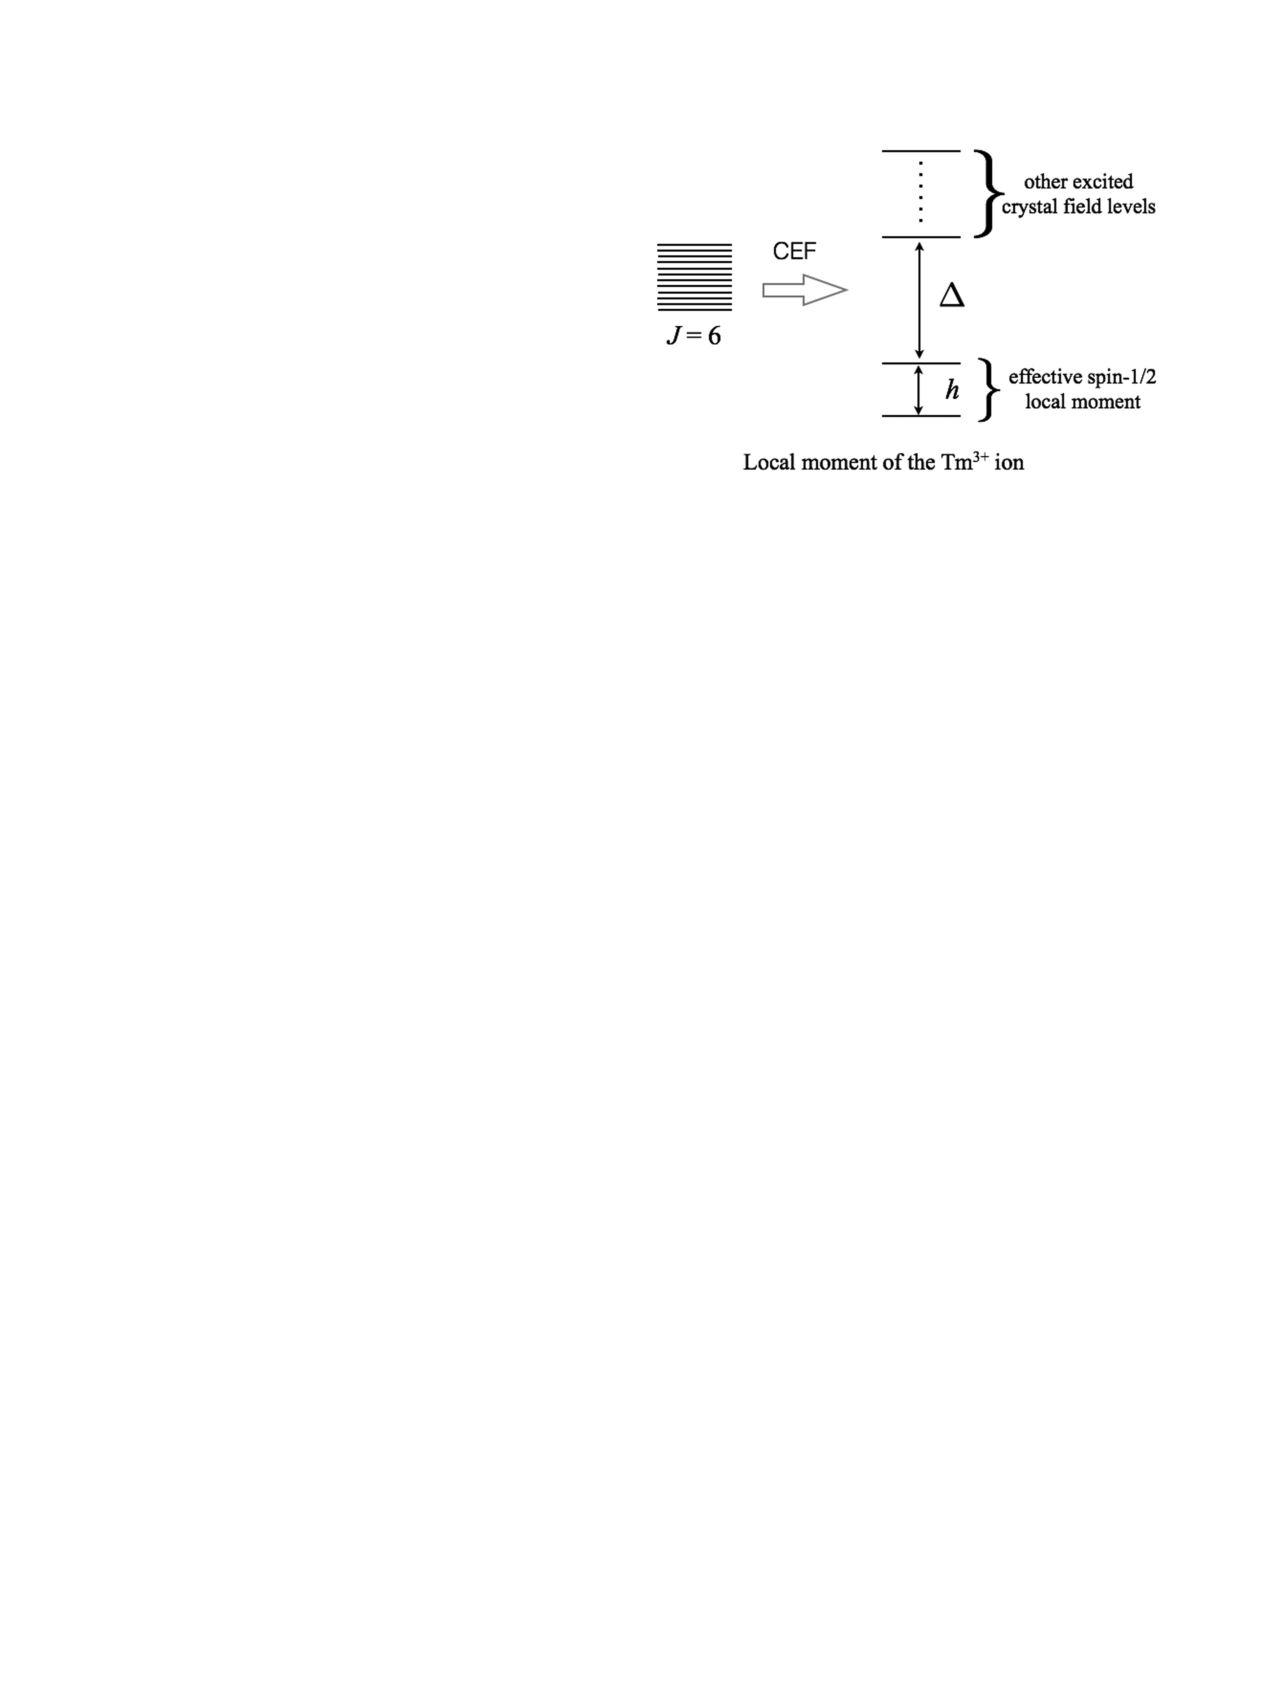
\includegraphics[width=\textwidth]{tm3+}

			{\small Changle Liu, Chun-Jiong Huang, and Gang Chen\\
			Phys. Rev. Research \textbf{2}, 043013 (2020).}
		\end{center}
		\column{.4\textwidth}
		\begin{itemize}
			\item Tm${}^{3+}$: $S=1$; no Kramers degeneracy.
			\item The two lowest levels of Tm${}^{3+}$ ion form an effective spin-$\frac12$.
			\item Dipole-multipole:
			\begin{align*}TS^{x,y}T^{-1}&=S^{x,y};\\
				TS^zT^{-1}&=-S^z.\end{align*}
		\end{itemize}
	\end{columns}
\end{frame}

\end{document}
% !TEX engine = xelatex
%%% Local Variables:
%%% coding: utf-8
%%% mode: latex
%%% TeX-engine: xetex
%%% End:
